
\subsection{Plateforme robotique}

\begin{frame}{Le robot Sigmaban (1/2) -- Caractéristiques matérielles}
    \begin{columns}
        \begin{column}{0.32\linewidth}
            Robot humanoïde Sigmaban :
            \begin{itemize}
                \item Taille : $57$~cm
                \item Poids : $4.2$~Kg
                \item Articulations : $20$
                \vspace{1.0em}
                \item Caméra industrielle
                \item Processeur x86
                \item IMU (accéléromètres, gyromètres)
                \item Capteurs de pression
                \item Servomoteurs Dynamixel
            \end{itemize}
        \end{column}
        \begin{column}{0.6\linewidth}
            \begin{columns}
                \begin{column}{0.4\linewidth}
                    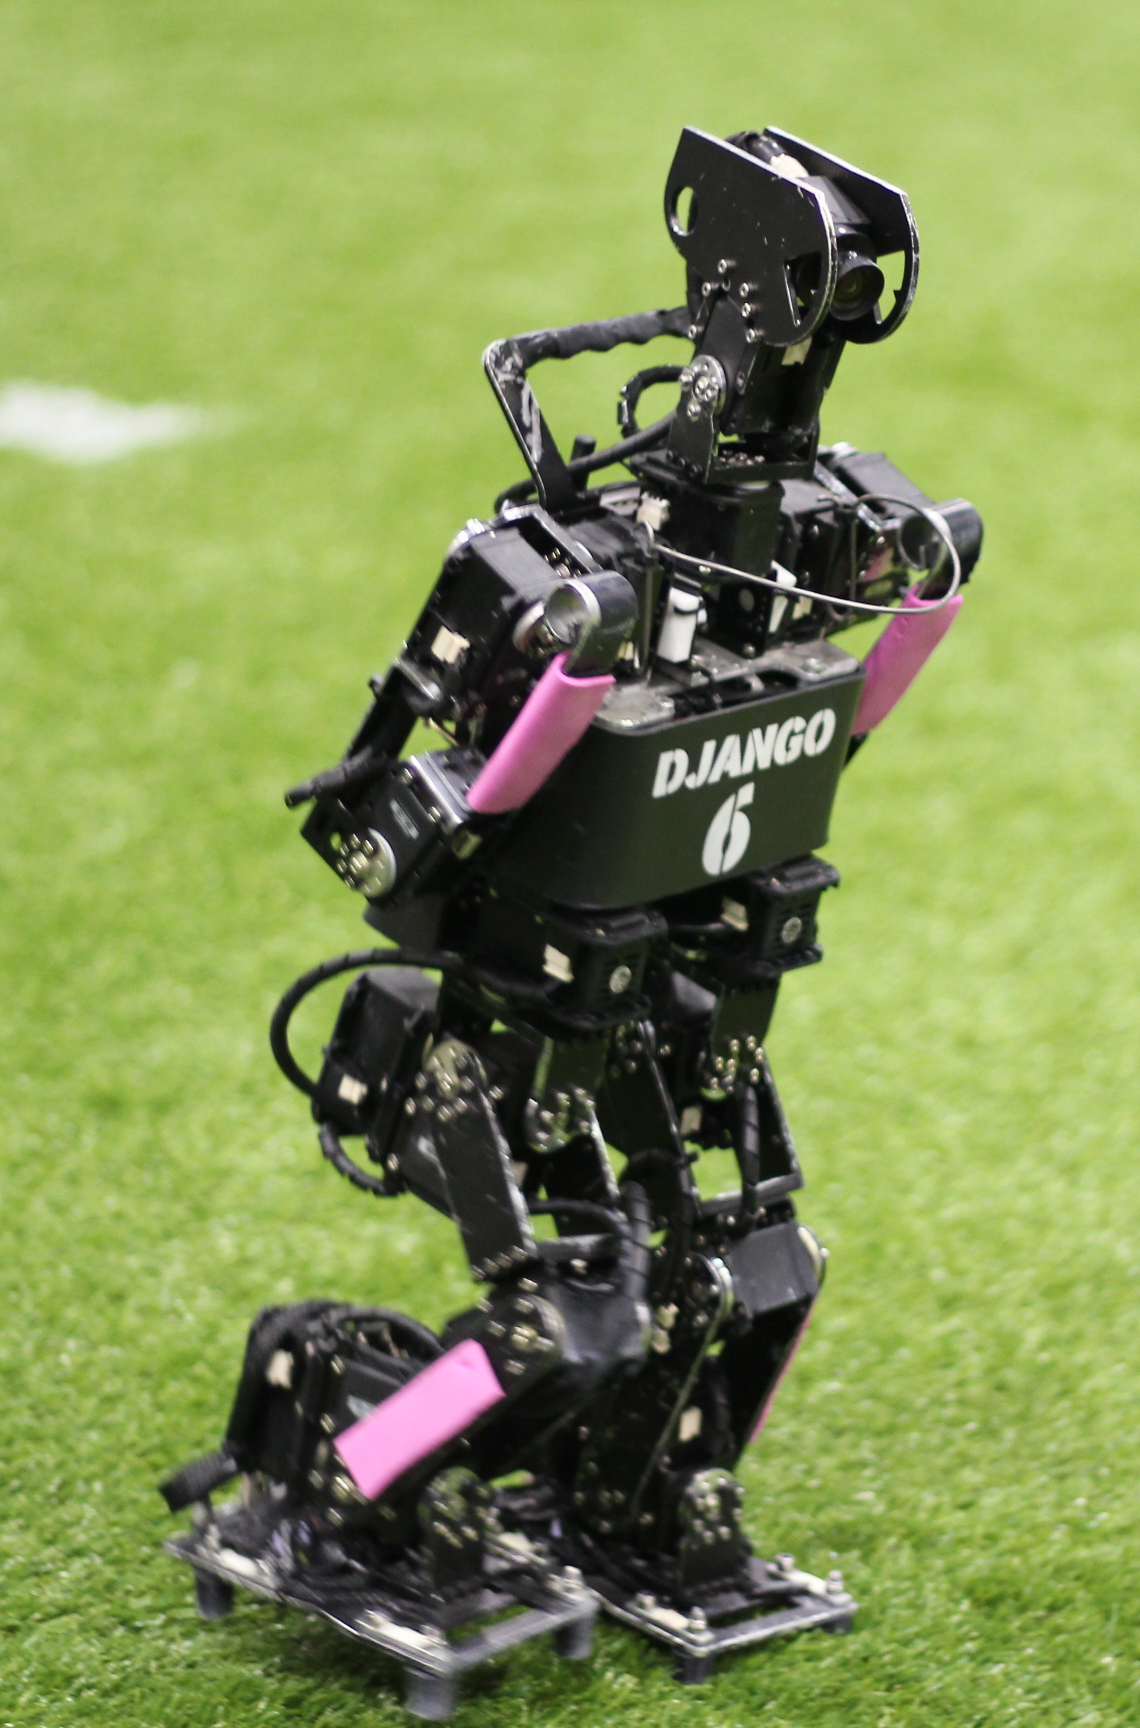
\includegraphics[width=1.0\linewidth]{../media/sigmaban_1_6.png}
                \end{column}
                \begin{column}{0.6\linewidth}
                    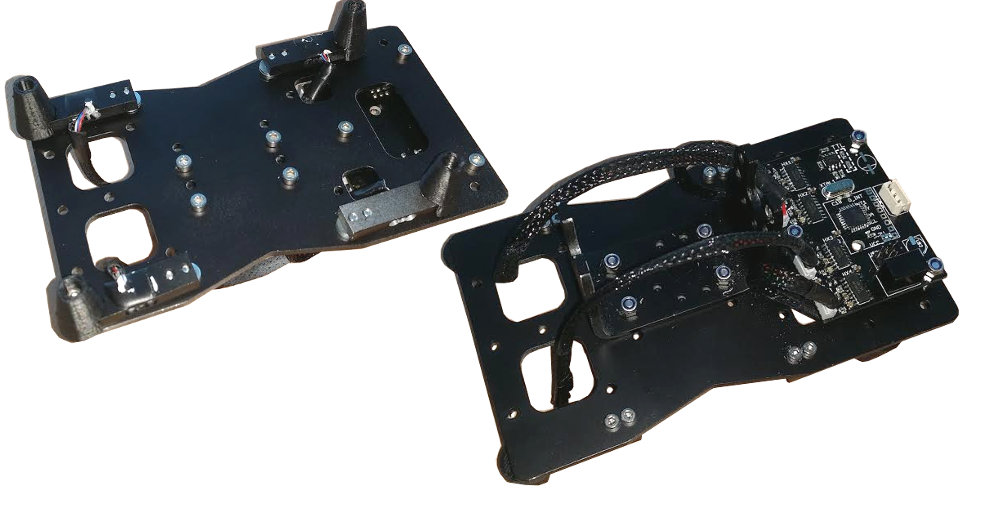
\includegraphics[width=1.1\linewidth]{../media/pressures2.png}
                    \newline
                    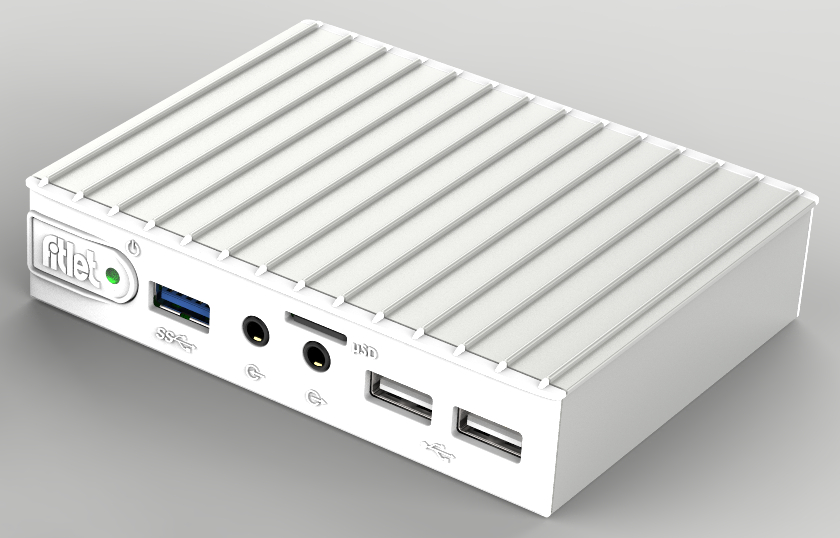
\includegraphics[width=0.5\linewidth]{../media/fitlet.jpg}
                    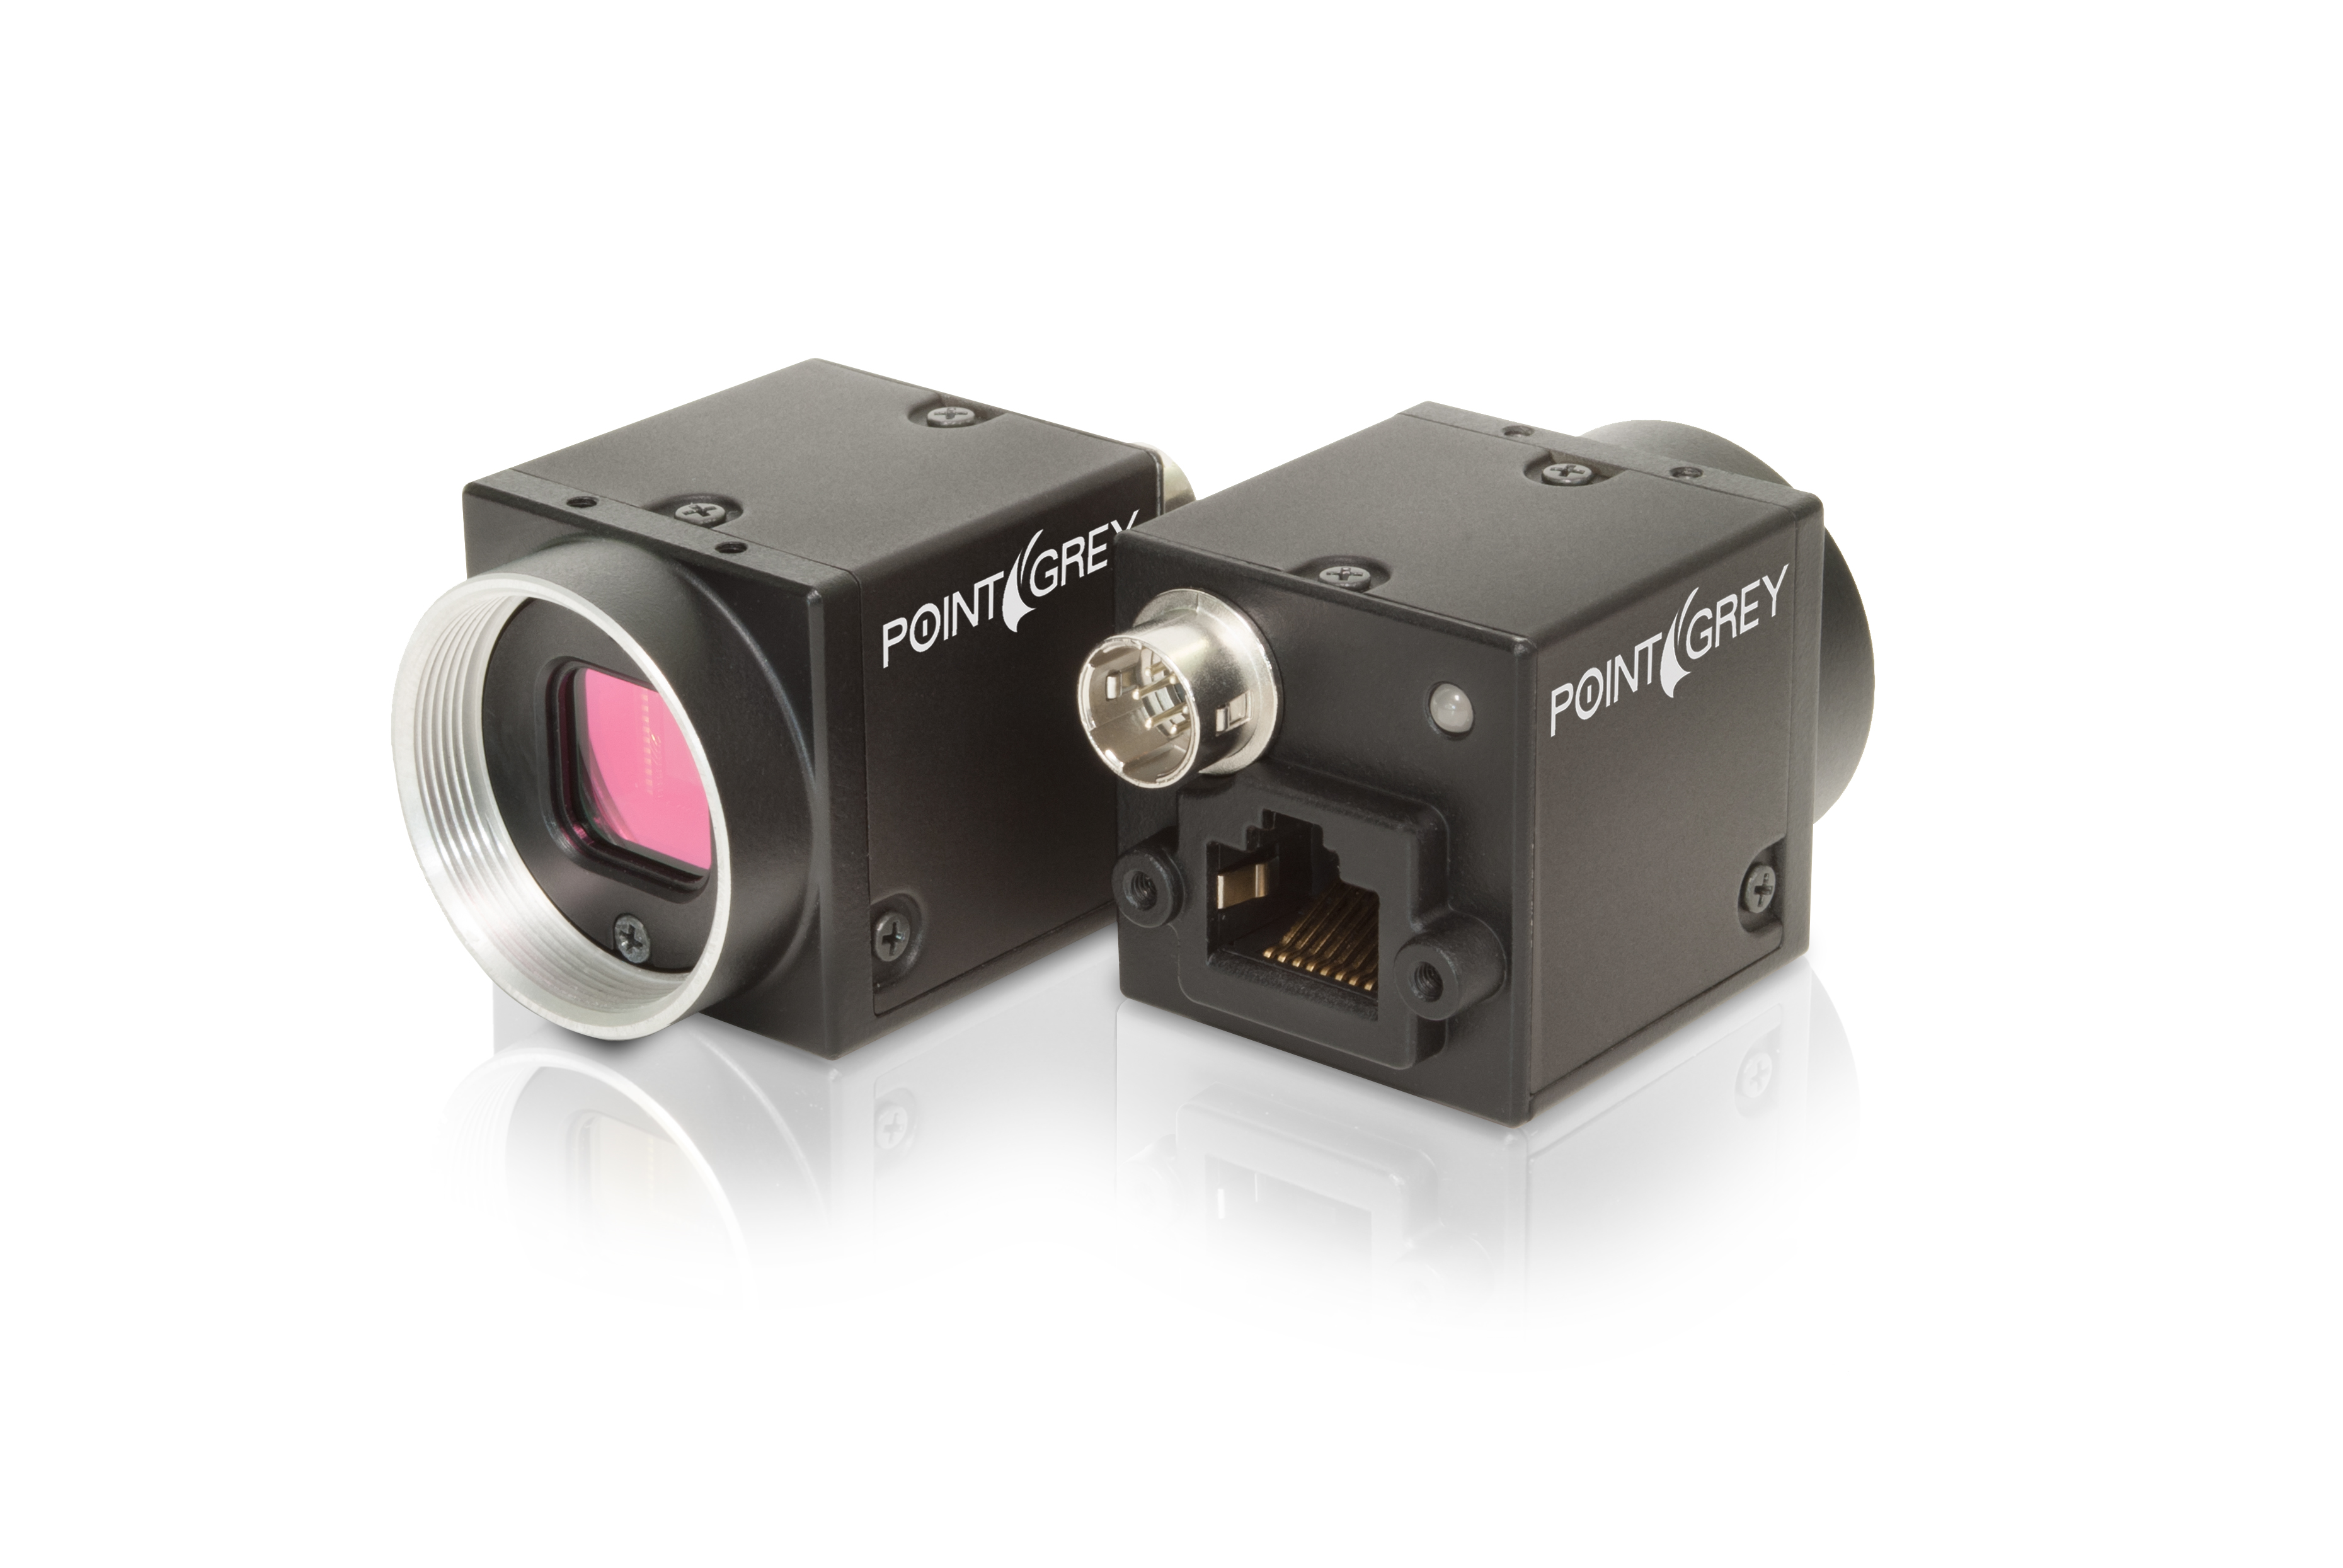
\includegraphics[width=0.6\linewidth]{../media/camera_blackfly.jpg}
                \end{column}
            \end{columns}
            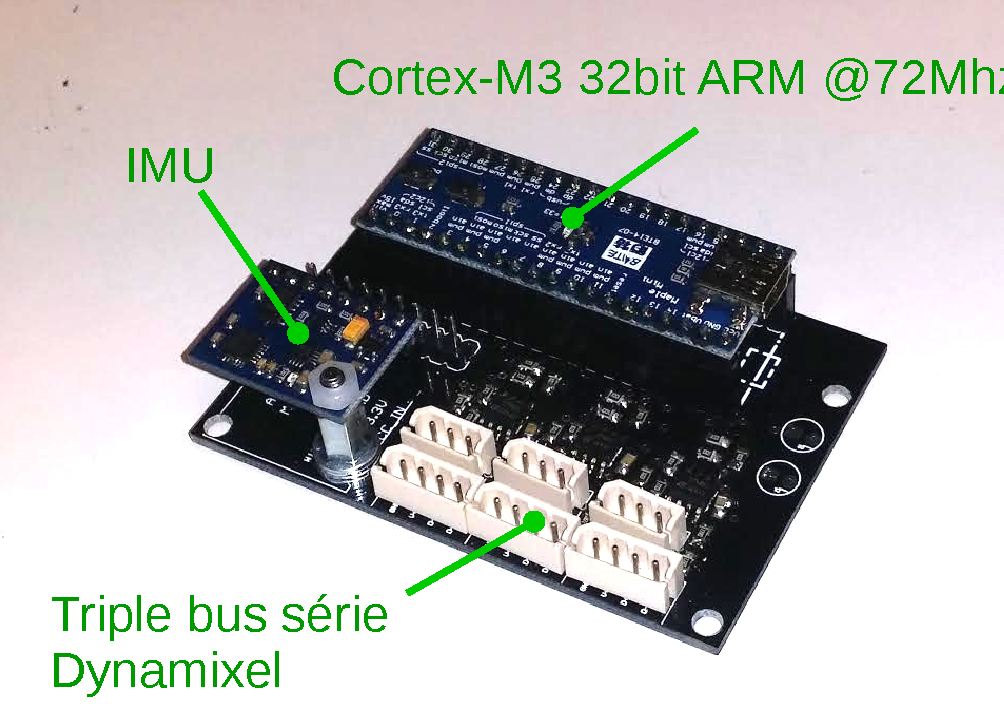
\includegraphics[type=pdf,ext=.pdf,read=.pdf,height=2cm]{../schema/3bus}
            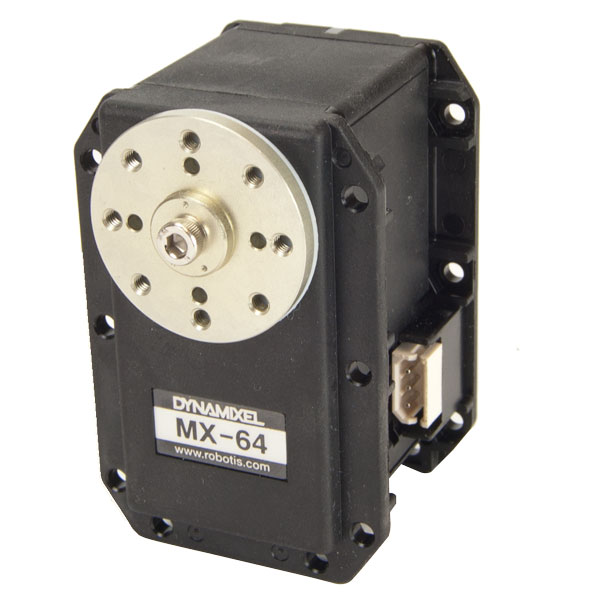
\includegraphics[height=2cm]{../media/dynamixel1.jpg}
            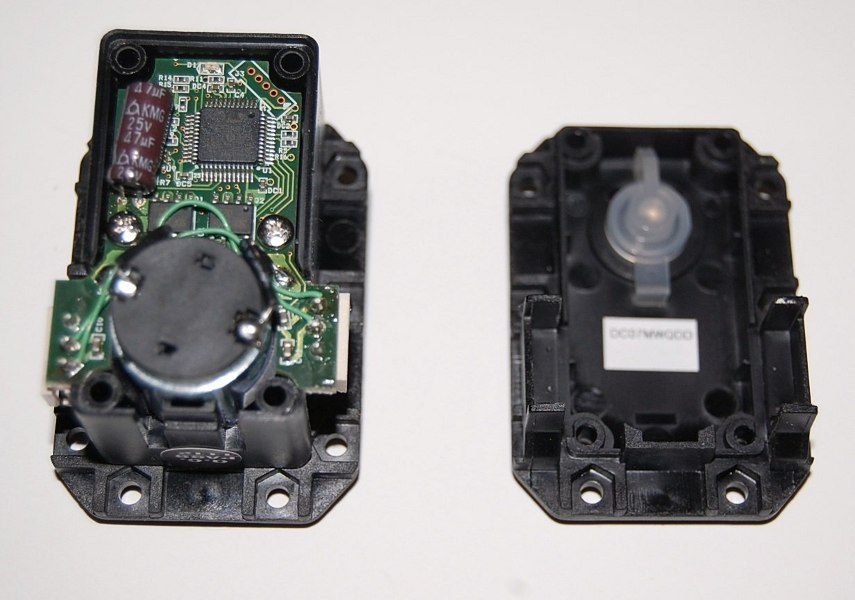
\includegraphics[height=2cm]{../media/dynamixel2.jpg}
        \end{column}
    \end{columns}
\end{frame}

\begin{frame}{Le robot Sigmaban (2/2) -- Robuste mais imparfait}
    \begin{columns}
        \begin{column}{0.55\linewidth}
            \begin{block}{Imperfections}
                Comportement réel $\neq$
                prédiction du modèle solide rigide
            \end{block}
            Robots humanoïdes précis :
            HRP-2, ASIMO, iCub (jambes), HOAP-3\\
            \vspace{1.0em}
            Nos robots :
            \begin{itemize}
                \item Coût moindre
                \item Nombreuses imperfections
                \item Matchs RoboCup : chocs importants, chutes fréquentes
                \item Robustes et solides
            \end{itemize}
        \end{column}
        \begin{column}{0.45\linewidth}
            \vspace{-1.2em}
            \begin{center}
            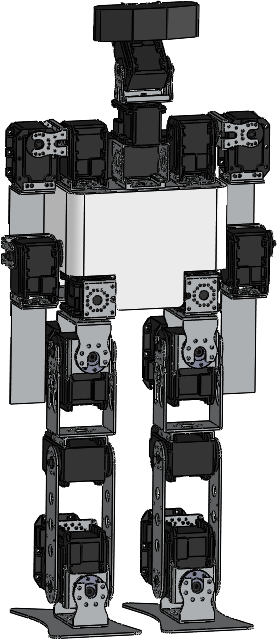
\includegraphics[height=2.9cm]{../media/sigmaban_cao2.png}
            \hspace{0.5cm}
            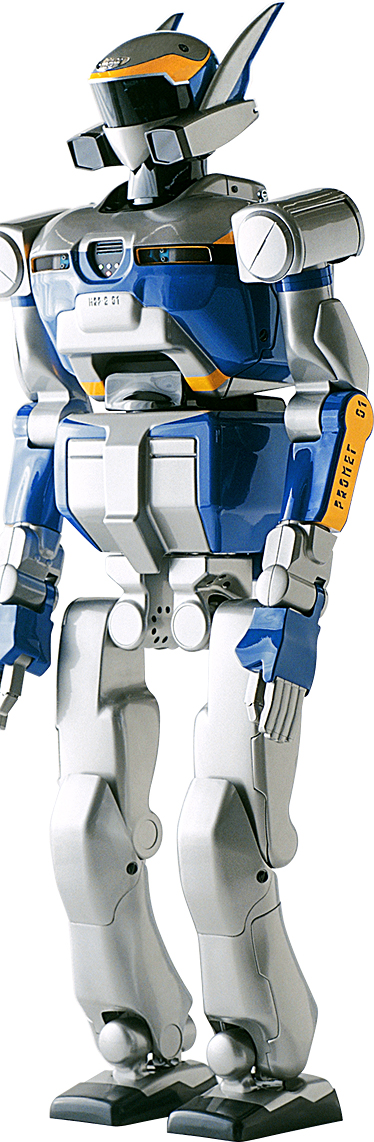
\includegraphics[height=8cm]{../media/hrp2.jpg}
            \newline
            \scriptsize
            (Source : Shuuji Kajita et al.)
            \end{center}
        \end{column}
    \end{columns}
\end{frame}

\begin{frame}{Imperfections (1/3) -- Déformations mécaniques}
    \begin{columns}
        \begin{column}{0.5\linewidth}
            \centering
            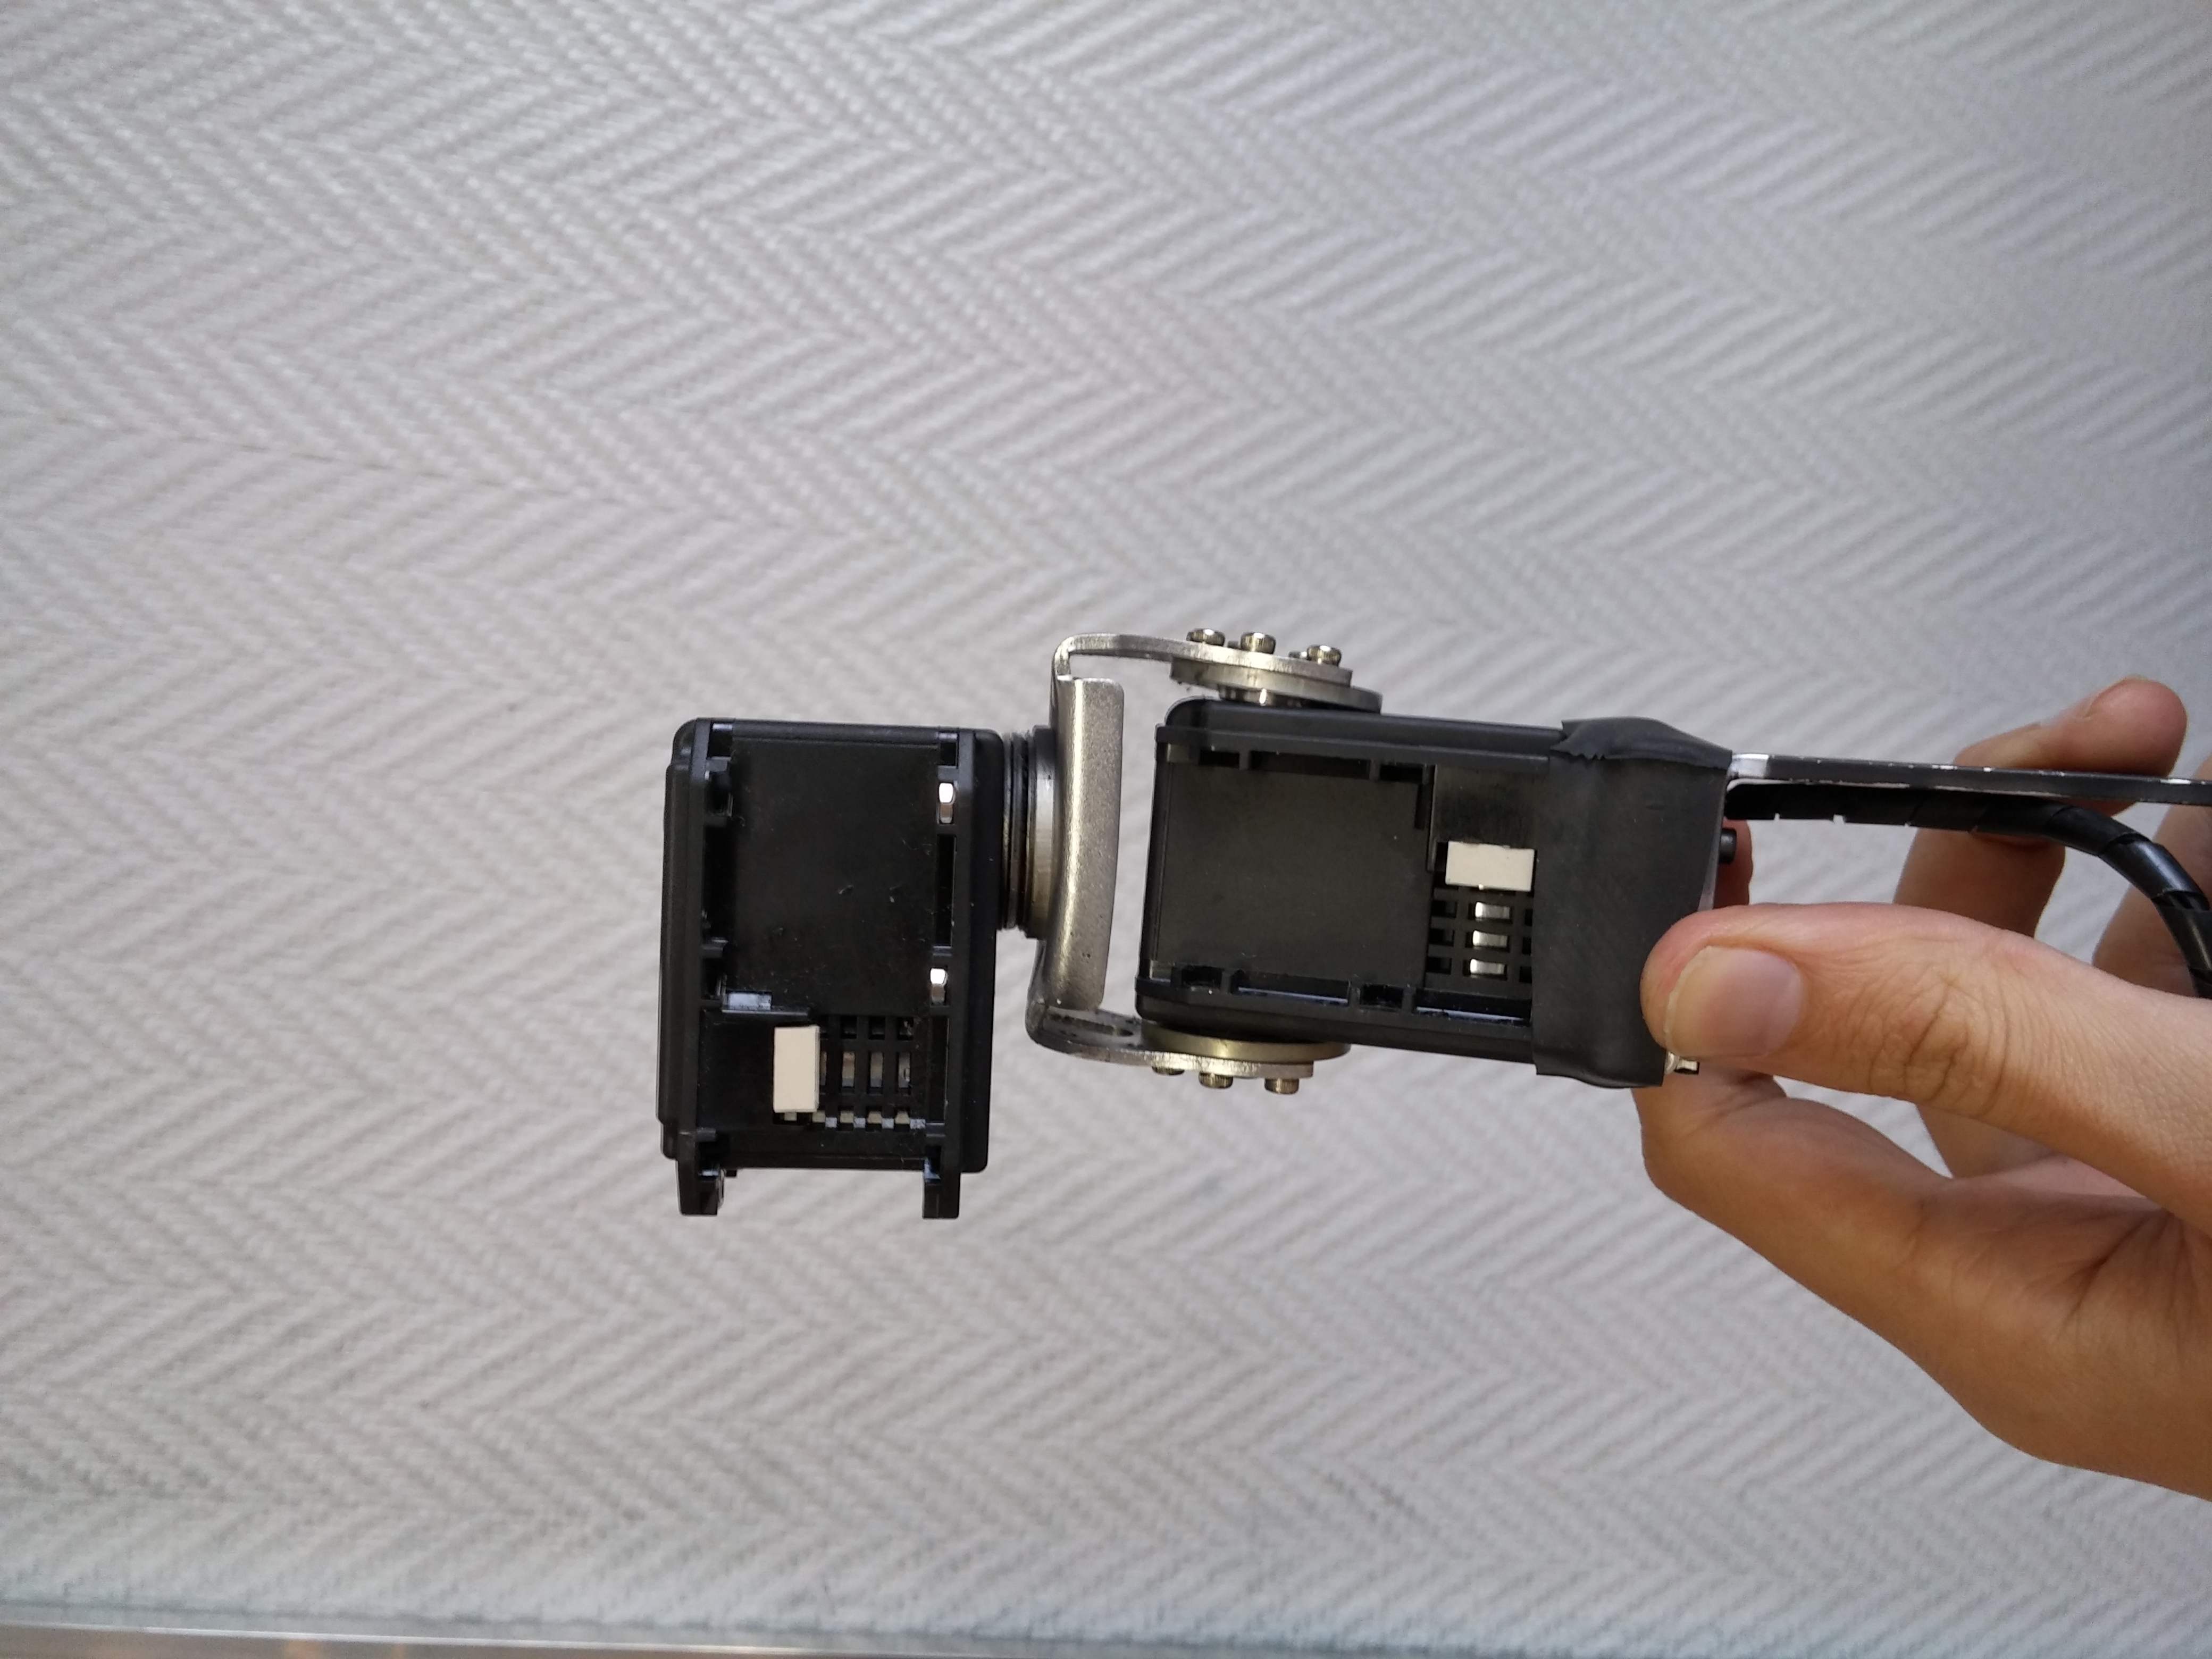
\includegraphics[height=4.5cm]{../media/torsion_meca1.jpg}
        \end{column}
        \begin{column}{0.5\linewidth}
            \centering
            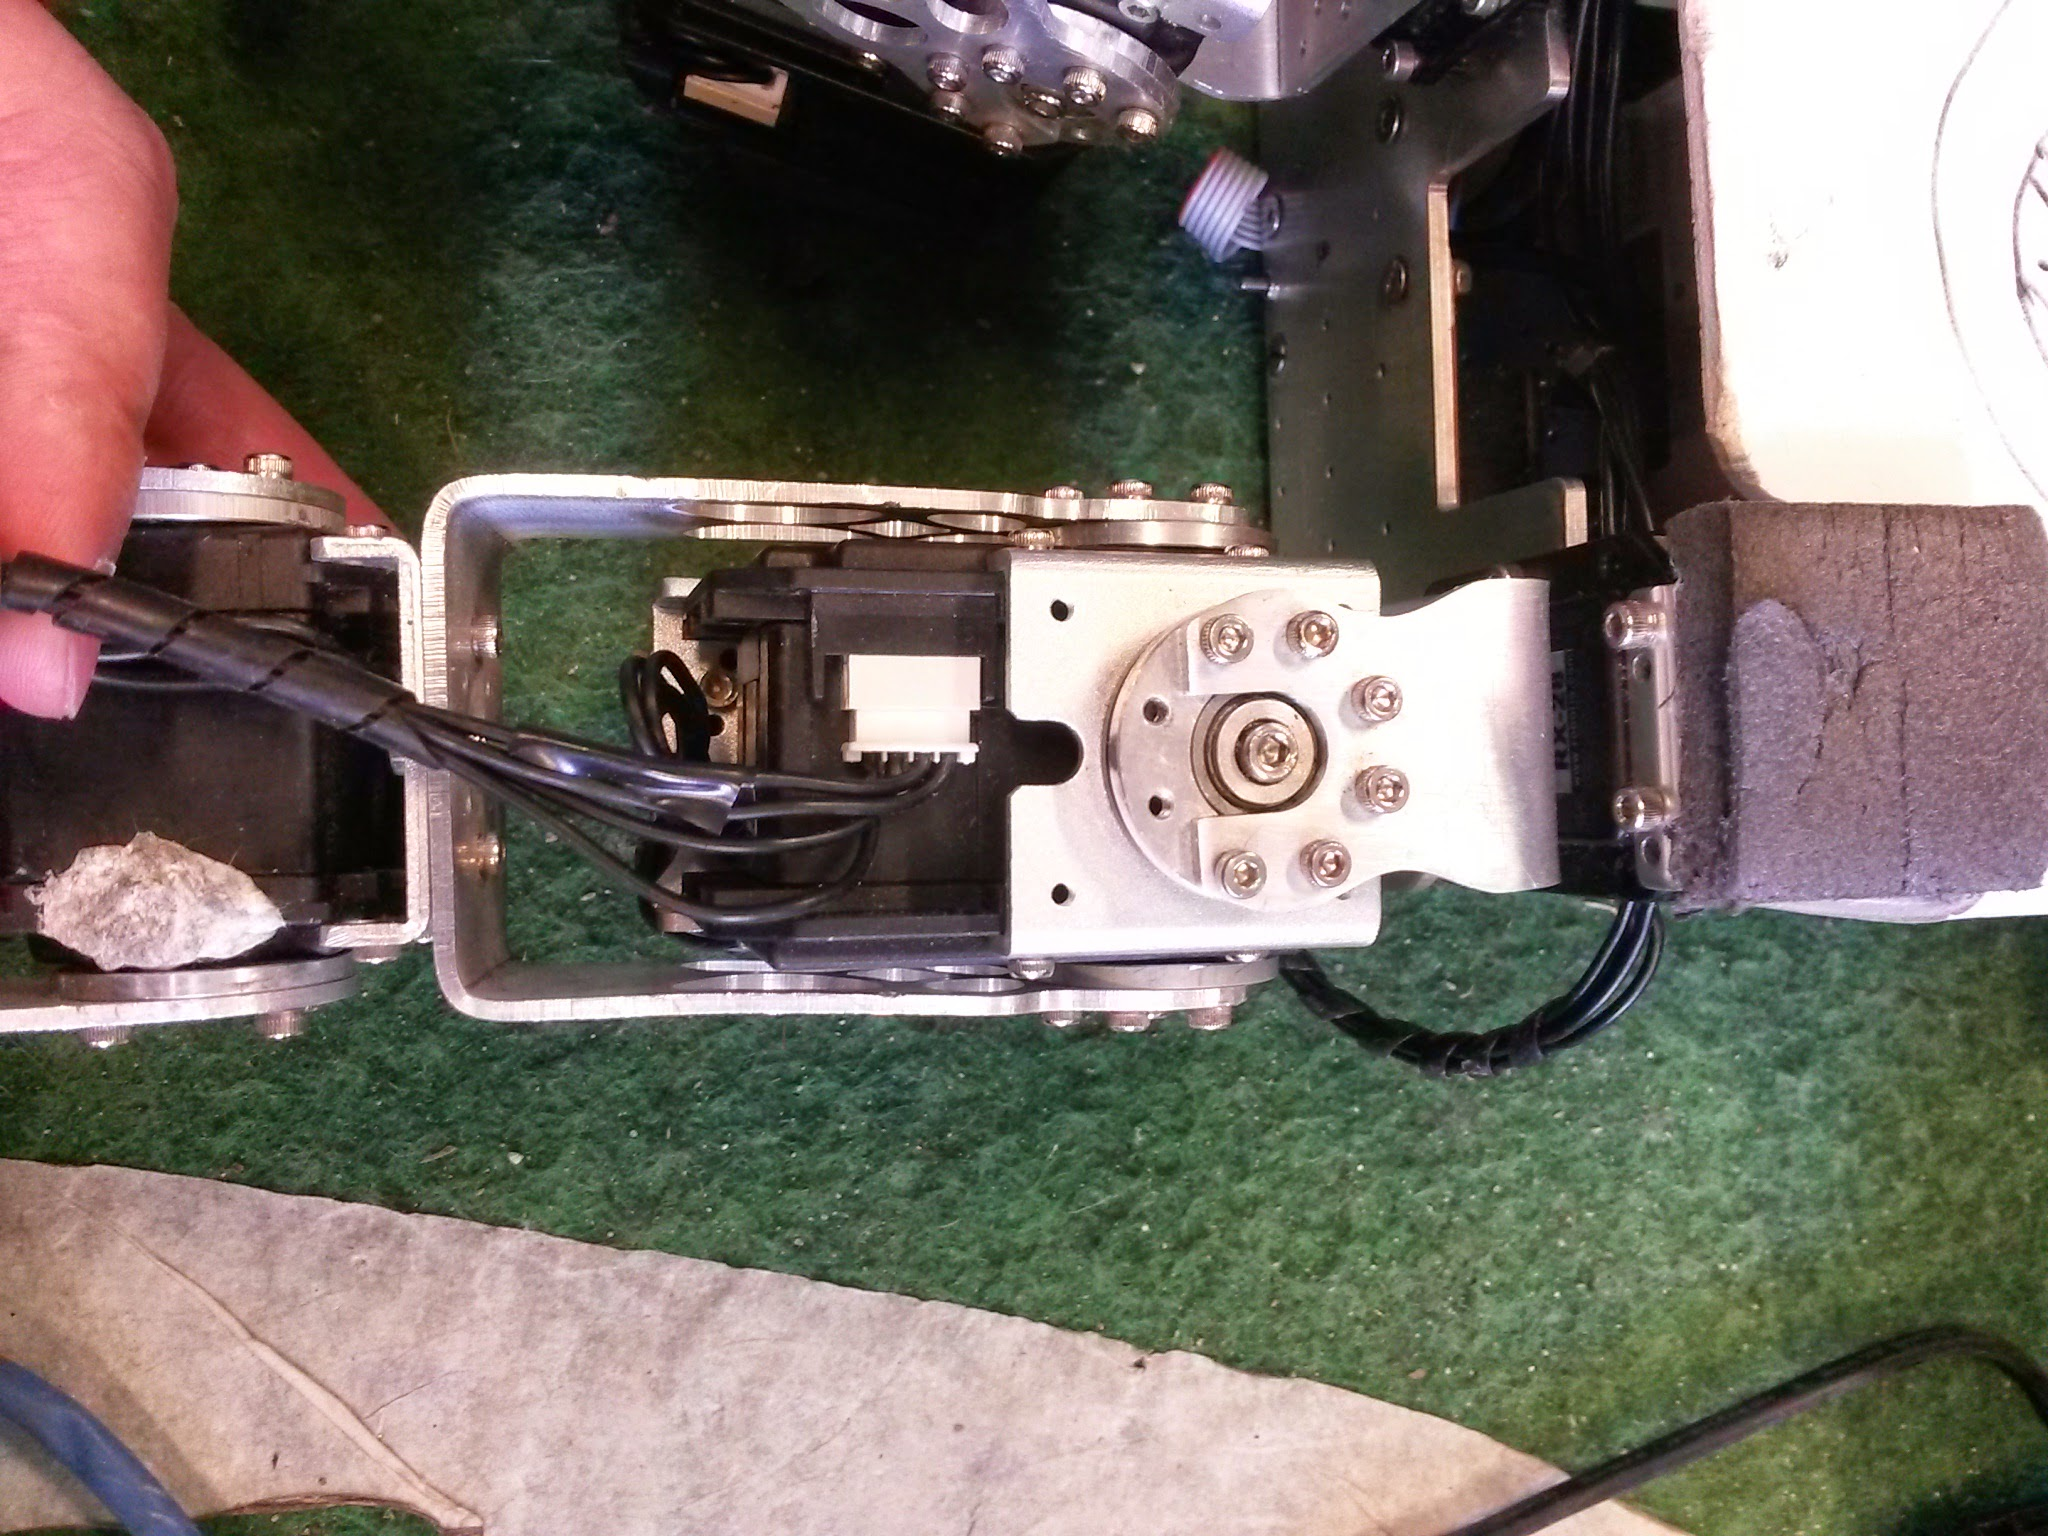
\includegraphics[height=4.5cm]{../media/torsion_meca2.jpg}
        \end{column}
    \end{columns}
    \vspace{1.0em}
    \begin{itemize}
        \item Segments mécaniques et torsions arbres moteur
        \item Usure : chutes et collisions
        \item Erreur statique du modèle géométrique
    \end{itemize}
\end{frame}

\begin{frame}{Imperfections (2/3) -- Jeu des engrenages}
    \begin{columns}
        \begin{column}{0.5\linewidth}
            \centering
            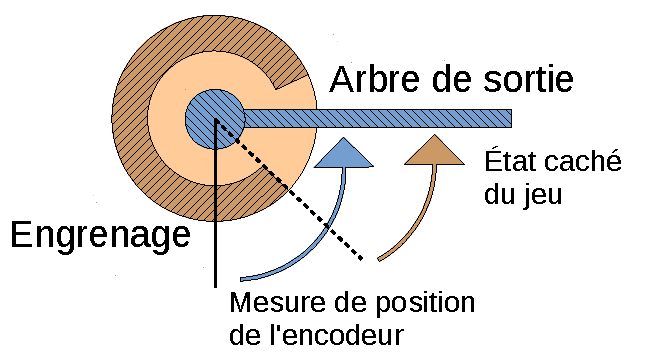
\includegraphics[type=pdf,ext=.pdf,read=.pdf,width=0.8\linewidth]{../schema/backlash_meca}
        \end{column}
        \begin{column}{0.5\linewidth}
            \centering
            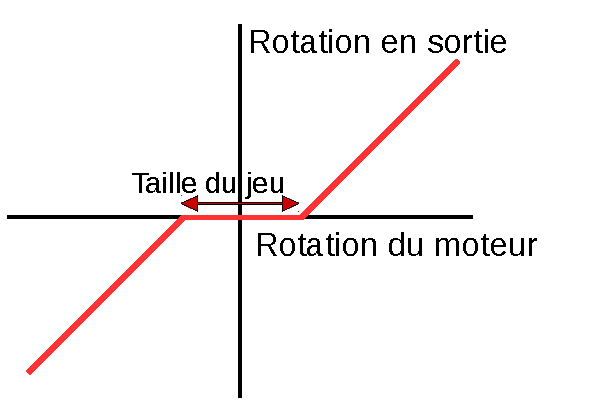
\includegraphics[type=pdf,ext=.pdf,read=.pdf,width=0.8\linewidth]{../schema/backlash_function}
        \end{column}
    \end{columns}
    \vspace{1.0em}
    \begin{itemize}
        \item Augmente avec l'âge du robot
        \item Mesuré par les encodeurs
        \item Affecte la dynamique
    \end{itemize}
\end{frame}

\begin{frame}{Imperfections (3/3) -- Asservissement des servomoteurs}
    \begin{columns}
        \begin{column}{0.5\linewidth}
            \begin{itemize}
                \item Asservissement réactif (proportionnel)
                \item Erreur angulaire > $10$\degres
            \end{itemize}
        \end{column}
        \begin{column}{0.5\linewidth}
            \centering
            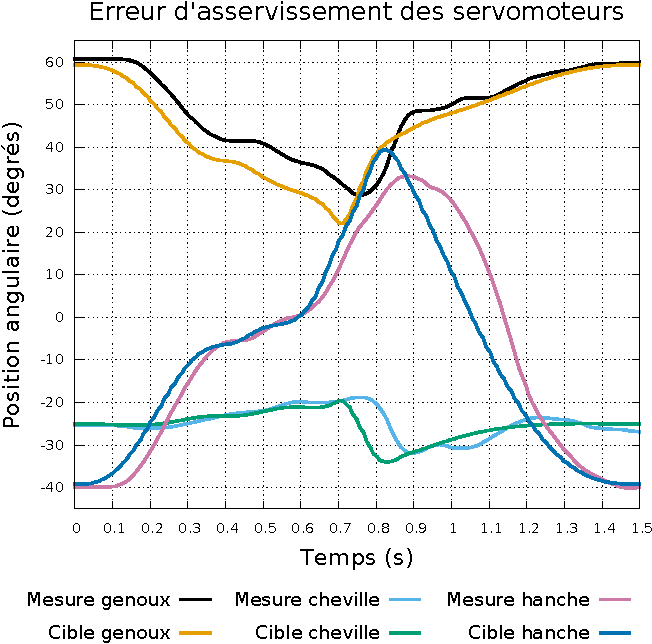
\includegraphics[type=pdf,ext=.pdf,read=.pdf,width=0.9\linewidth]{../plot/motors_control}
        \end{column}
    \end{columns}
    Pré-compensation (\textit{feedforward}) :
    \begin{block}{}
        \customtextcolor{
            \small
            \textit{Dynaban, an open-source alternative firmware for dynamixel servomotors}}\\
        \scriptsize
        Rémi Fabre, Quentin Rouxel, Grégoire Passault, Steve N'Guyen, Olivier Ly\\
        Symposium RoboCup, 2016\\
    \end{block}
    $\Rightarrow$ Pas utilisé dans la suite
\end{frame}

